\documentclass[12pt,a4paper]{article}
\usepackage[spanish,es-tabla]{babel}
\usepackage{bbm}
\usepackage[utf8]{inputenc}
\usepackage{multicol}
\usepackage[T1]{fontenc}
\usepackage{graphicx}
\usepackage{gensymb}
\usepackage{amssymb, amsmath} %Paquetes matemáticos de la American Mathematical Society
\parskip=1 mm
\oddsidemargin -0.8 cm
\headsep -2 cm
\textwidth=17.8cm
\textheight=25.5cm
\begin{document}
\title{Laboratorio de Mecánica, Práctica 10 - Segunda Ley de Newton}
\date{28 de abril del 2025}
\author{\textbf{Ortega Montero Fernando Naed} - Equipo 4\\
Yibran Morales Munguía\\
Victor Manuel Santillan Romero}
\maketitle
\section{Resumen}

Este informe tratara de encontrar la fuerza que se aplica sobre un objeto conociendo su peso y su aceleración gracias a la Segunda Ley de Newton. 

\section{Introducción}

La Segunda Ley de Newton relaciona el producto de la masa y la aceleración de un objeto con la suma de fuerzas que actúan sobre él.

\[\sum F = m a\]

En el modelo ideal de este experimento tenemos un sistema de dos objetos atados a una cuerda rígida y sin masa, donde la fuerza que actúa sobre el sistema es la fuerza de gravedad, si obtenemos las ecuaciones de nuestro sistema estas serian.

\[mg = Ma\]

Donde…\\
m = masa del objeto A, el objeto afectado por la gravedad.\\
g = aceleración de la gravedad.\\
M = masa del objeto B, el objeto que recibe la fuerza del objeto A .\\
a = aceleración del objeto B.\\

Así mismo se tienen que mencionar la ecuación de la posición con respecto del tiempo la cual es: 
\[ x(t) = x_0 + v_0 t + \frac{1}{2}a t^2\]

Donde…\\
$x(t)$ = Posición en el tiempo t, en metros (m)\\
$x_0$ = Posición inicial, en metros (m)\\
$v_0$ =Velocidad inicial, en metros sobre segundos ($\frac{m}{s}$)\\
$a$ = Aceleración, en metros sobre segundo al cuadrado ($\frac{m}{s^2}$)\\
$t$ = tiempo


\section{Desarrollo experimental}

Se colocó un riel de aire en posición horizontal, a un extremo de una cuerda se amarró el carro para riel, al otro extremo se amarró una pesa, y con ayuda de una polea en un extremo del riel se hizo colgar la masa en posición horizontal para que la gravedad realizara la fuerza contra la masa. 
Se soltó el carro desde una distancia arbitraria y se tomo un video del movimiento, este video se analizó utilizando el software Traker con el objetivo de analizar la aceleración del objeto. 

Nótese que el objeto empieza con $v_0 = 0 \frac{m}{s}$ y $x_0 = 0 m$ por lo que las ecuaciones de movimiento se reducen a solo...
\[x(t) = \frac{1}{2} a t^2\]

Por lo que, cuando se aplique el cambio de variable y la regresión lineal, la pendiente de la recta será $\frac{1}{2}a = m$, por lo que la aceleración será $a = 2m$.

\section{Resultados}

En la Tabla 1 se exponen los resultados obtenidos experimentalmente de la posición con respecto del tiempo de un objeto acelerado por una masa de 20 g así como el cambio de variable de $T = t^2$ para la regresión lineal, en la Tabla 2 se exponen los resultados de la regresión lineal para la Tabla 1.\\ 
En la Tabla 3 se exponen los resultados obtenidos experimentalmente de la posición con respecto del tiempo de un objeto acelerado por una masa de 50 g así como el cambio de variable de $T = t^2$ para la regresión lineal, en la Tabla 4 se exponen los resultados de la regresión lineal para la Tabla 3. \\

\subsection{Obtencion de incertidumbres}

Se obtiene la incertidumbre de la velocidad haciendo uso de las siguientes ecuaciones:

\[S_y = \sqrt{\frac{\sum_{i=1}^N (y_i - mx_i - b)^2}{N-2}}\] 

\[S_m = S_y \sqrt{\frac{N}{N\sum_{i=1}^N x_i^2 - \left(\sum_{i=1}^N  x_i\right)^2}}\]

Donde $y = x$, $x = t$, $b = x_0$ y el resto de valores necesarios se exponen en las Tablas 3 y 4 junto con los resultados de $S_x$ y $S_v$\\

\[S_x = \sqrt{\frac{\sum_{i=1}^{N}(x_i - vt_i - x_0)^2}{8}}\] 

\[S_a = S_x \sqrt{\frac{N}{N\sum_{i=1}^{N} t_i^2 - \left(\sum_{i=1}^{N}  t_i\right)^2}}\]

Así mismo para calcular la incertidumbre de la Fuerza se hace uso de la ley de la propagación de la incertidumbre cuya ecuación es…

\[S_c^2(y) = \sum^k_{i=1} \left(\frac{\partial f}{\partial x_i}\right)^2 S^2(x_i)\]  

Donde, y = F, cuya única variable independiente de la Fuerza es la aceleración, por lo que la derivada total de la Fuerza con respecto de la aceleración es…

\[\frac{dF}{da} = m\]

Por lo que la incertidumbre de la Fuerza es:

\[S_F = m \cdot S_a\]

\clearpage

\begin{table}[h!]
\begin{center}
\begin{tabular}{|c|c|c|}
\hline
tiempo (s) & $T = t^2$ ($s^2$) & posición (m) \\ \hline
0.000 (0.001) s & 0.000 (0.001) $s^2$ & 0.000 (0.001) m \\ \hline
0.042 (0.001) s & 0.002 (0.001) $s^2$ & 0.005 (0.001) m \\ \hline
0.083 (0.001) s & 0.007 (0.001) $s^2$ & 0.011 (0.001) m \\ \hline
0.125 (0.001) s & 0.016 (0.001) $s^2$ & 0.019 (0.001) m \\ \hline
0.167 (0.001) s & 0.028 (0.001) $s^2$ & 0.026 (0.001) m \\ \hline
0.208 (0.001) s & 0.043 (0.001) $s^2$ & 0.035 (0.001) m \\ \hline
0.250 (0.001) s & 0.062 (0.001) $s^2$ & 0.046 (0.001) m \\ \hline
0.292 (0.001) s & 0.085 (0.001) $s^2$ & 0.058 (0.001) m \\ \hline
0.333 (0.001) s & 0.111 (0.001) $s^2$ & 0.071 (0.001) m \\ \hline
0.375 (0.001) s & 0.141 (0.001) $s^2$ & 0.084 (0.001) m \\ \hline
0.417 (0.001) s & 0.174 (0.001) $s^2$ & 0.097 (0.001) m \\ \hline
0.458 (0.001) s & 0.210 (0.001) $s^2$ & 0.114 (0.001) m \\ \hline
0.500 (0.001) s & 0.250 (0.001) $s^2$ & 0.129 (0.001) m \\ \hline
0.542 (0.001) s & 0.294 (0.001) $s^2$ & 0.146 (0.001) m \\ \hline
0.583 (0.001) s & 0.340 (0.001) $s^2$ & 0.167 (0.001) m \\ \hline
0.625 (0.001) s & 0.391 (0.001) $s^2$ & 0.185 (0.001) m \\ \hline
0.666 (0.001) s & 0.444 (0.001) $s^2$ & 0.205 (0.001) m \\ \hline
0.708 (0.001) s & 0.501 (0.001) $s^2$ & 0.229 (0.001) m \\ \hline
0.750 (0.001) s & 0.562 (0.001) $s^2$ & 0.249 (0.001) m \\ \hline
0.791 (0.001) s & 0.626 (0.001) $s^2$ & 0.274 (0.001) m \\ \hline
0.833 (0.001) s & 0.694 (0.001) $s^2$ & 0.300 (0.001) m \\ \hline
0.875 (0.001) s & 0.766 (0.001) $s^2$ & 0.324 (0.001) m \\ \hline
0.916 (0.001) s & 0.839 (0.001) $s^2$ & 0.349 (0.001) m \\ \hline
0.958 (0.001) s & 0.918 (0.001) $s^2$ & 0.376 (0.001) m \\ \hline
1.000 (0.001) s & 1.000 (0.001) $s^2$ & 0.406 (0.001) m \\ \hline
1.041 (0.001) s & 1.084 (0.001) $s^2$ & 0.436 (0.001) m \\ \hline
1.083 (0.001) s & 1.173 (0.001) $s^2$ & 0.466 (0.001) m \\ \hline
1.125 (0.001) s & 1.266 (0.001) $s^2$ & 0.499 (0.001) m \\ \hline
1.166 (0.001) s & 1.360 (0.001) $s^2$ & 0.533 (0.001) m \\ \hline
1.208 (0.001) s & 1.459 (0.001) $s^2$ & 0.567 (0.001) m \\ \hline
1.250 (0.001) s & 1.562 (0.001) $s^2$ & 0.601 (0.001) m \\ \hline
1.291 (0.001) s & 1.667 (0.001) $s^2$ & 0.637 (0.001) m \\ \hline
1.333 (0.001) s & 1.777 (0.001) $s^2$ & 0.673 (0.001) m \\ \hline
1.375 (0.001) s & 1.891 (0.001) $s^2$ & 0.713 (0.001) m \\ \hline
1.416 (0.001) s & 2.005 (0.001) $s^2$ & 0.751 (0.001) m \\ \hline
1.458 (0.001) s & 2.126 (0.001) $s^2$ & 0.792 (0.001) m \\ \hline
1.500 (0.001) s & 2.250 (0.001) $s^2$ & 0.833 (0.001) m \\ \hline
1.541 (0.001) s & 2.375 (0.001) $s^2$ & 0.874 (0.001) m \\ \hline
1.583 (0.001) s & 2.506 (0.001) $s^2$ & 0.923 (0.001) m \\ \hline
1.625 (0.001) s & 2.641 (0.001) $s^2$ & 0.967 (0.001) m \\ \hline
1.666 (0.001) s & 2.776 (0.001) $s^2$ & 1.006 (0.001) m \\ \hline

\end{tabular}
\caption{Tiempos - Cambio de variable - Posición con una masa de 20 g}
\end{center}
\end{table}



\begin{table}[h!]
\begin{center}
\begin{tabular}{|c|c|}
\hline
Cantidad & Valor \\ \hline
$ \sum^{10}_{i = 1} t_i $ & 34.158 \\ \hline
$\sum^{10}_{i = 1} t_i^2$ & 38.417 \\ \hline
$\sum^{10}_{i = 1} x_i$ & 15.176 \\ \hline
$\sum^{10}_{i = 1} tx_i$ & 18.670 \\ \hline
m & 0.3588 \\ \hline
a = 2m & 0.7176 \\ \hline
$x_0$ & 0.034 \\ \hline
$S_x$ & 0.146 \\ \hline
$S_a$ & 0.0463 \\ \hline

\end{tabular}
\caption{Resultados de la regresión lineal de la Tabla 1}
\end{center}
\end{table}

\begin{figure}[h!]
\centering
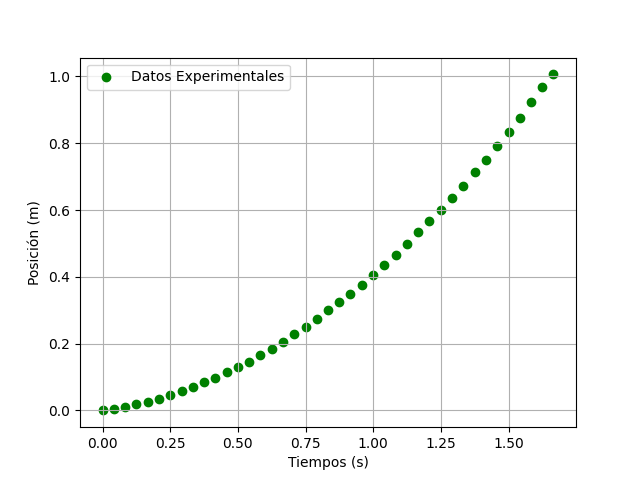
\includegraphics[scale=1]{20 g.png}
\caption{Grafica de la Tabla 1}
\end{figure}

\begin{figure}[h!]
\centering
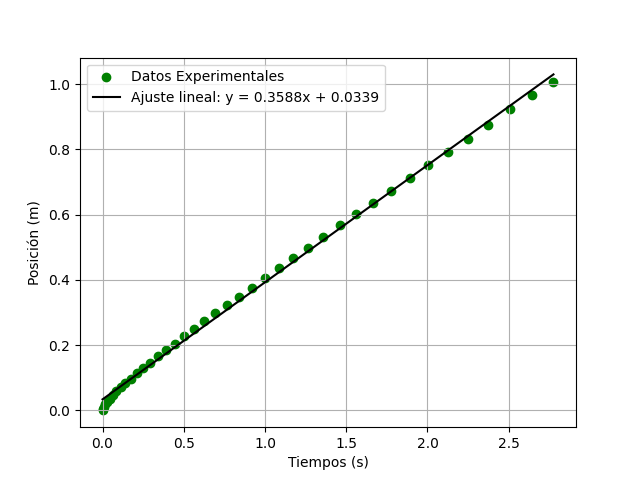
\includegraphics[scale=1]{20 g r.png}
\caption{Grafica de $t^2$ - posición con regresión lineal de la Tabla 1}
\end{figure}

\clearpage

\begin{table}[h!]
\begin{center}
\begin{tabular}{|c|c|c|}
\hline
tiempo (s) & $T = t^2$ ($s^2$) & posición (m) \\ \hline
0.000 (0.001) s & 0.000 (0.001) $s^2$ & 0.000 (0.001) m \\ \hline
0.042 (0.001) s & 0.002 (0.001) $s^2$ & 0.004 (0.001) m \\ \hline
0.083 (0.001) s & 0.007 (0.001) $s^2$ & 0.011 (0.001) m \\ \hline
0.125 (0.001) s & 0.016 (0.001) $s^2$ & 0.019 (0.001) m \\ \hline
0.167 (0.001) s & 0.028 (0.001) $s^2$ & 0.030 (0.001) m \\ \hline
0.208 (0.001) s & 0.043 (0.001) $s^2$ & 0.043 (0.001) m \\ \hline
0.250 (0.001) s & 0.062 (0.001) $s^2$ & 0.060 (0.001) m \\ \hline
0.292 (0.001) s & 0.085 (0.001) $s^2$ & 0.079 (0.001) m \\ \hline
0.333 (0.001) s & 0.111 (0.001) $s^2$ & 0.096 (0.001) m \\ \hline
0.375 (0.001) s & 0.141 (0.001) $s^2$ & 0.121 (0.001) m \\ \hline
0.417 (0.001) s & 0.174 (0.001) $s^2$ & 0.146 (0.001) m \\ \hline
0.458 (0.001) s & 0.210 (0.001) $s^2$ & 0.173 (0.001) m \\ \hline
0.500 (0.001) s & 0.250 (0.001) $s^2$ & 0.203 (0.001) m \\ \hline
0.542 (0.001) s & 0.294 (0.001) $s^2$ & 0.236 (0.001) m \\ \hline
0.583 (0.001) s & 0.340 (0.001) $s^2$ & 0.269 (0.001) m \\ \hline
0.625 (0.001) s & 0.391 (0.001) $s^2$ & 0.306 (0.001) m \\ \hline
0.666 (0.001) s & 0.444 (0.001) $s^2$ & 0.345 (0.001) m \\ \hline
0.708 (0.001) s & 0.501 (0.001) $s^2$ & 0.388 (0.001) m \\ \hline
0.750 (0.001) s & 0.562 (0.001) $s^2$ & 0.429 (0.001) m \\ \hline
0.791 (0.001) s & 0.626 (0.001) $s^2$ & 0.476 (0.001) m \\ \hline
0.833 (0.001) s & 0.694 (0.001) $s^2$ & 0.526 (0.001) m \\ \hline
0.875 (0.001) s & 0.766 (0.001) $s^2$ & 0.574 (0.001) m \\ \hline
0.916 (0.001) s & 0.839 (0.001) $s^2$ & 0.627 (0.001) m \\ \hline
0.958 (0.001) s & 0.918 (0.001) $s^2$ & 0.684 (0.001) m \\ \hline
1.000 (0.001) s & 1.000 (0.001) $s^2$ & 0.741 (0.001) m \\ \hline
1.041 (0.001) s & 1.084 (0.001) $s^2$ & 0.807 (0.001) m \\ \hline
1.083 (0.001) s & 1.173 (0.001) $s^2$ & 0.865 (0.001) m \\ \hline
1.125 (0.001) s & 1.266 (0.001) $s^2$ & 0.933 (0.001) m \\ \hline
1.166 (0.001) s & 1.360 (0.001) $s^2$ & 1.002 (0.001) m \\ \hline

\end{tabular}
\caption{Tiempos - Cambio de variable - Posición con una masa de 50 g}
\end{center}
\end{table}



\begin{table}[h!]
\begin{center}
\begin{tabular}{|c|c|}
\hline
Cantidad & Valor \\ \hline
$ \sum^{10}_{i = 1} t_i $ & 16.912 \\ \hline
$\sum^{10}_{i = 1} t_i^2$ & 13.384 \\ \hline
$\sum^{10}_{i = 1} x_i$ & 10.193 \\ \hline
$\sum^{10}_{i = 1} tx_i$ & 8.959 \\ \hline
m & 0.7305 \\ \hline
a = 2m & 1.461 \\ \hline
$x_0$ & 0.014 \\ \hline
$S_x$ & 0.128 \\ \hline
$S_a$ & 0.0682 \\ \hline

\end{tabular}
\caption{Resultados de la regresión lineal de la Tabla 3}
\end{center}
\end{table}

\clearpage

\begin{figure}[h!]
\centering
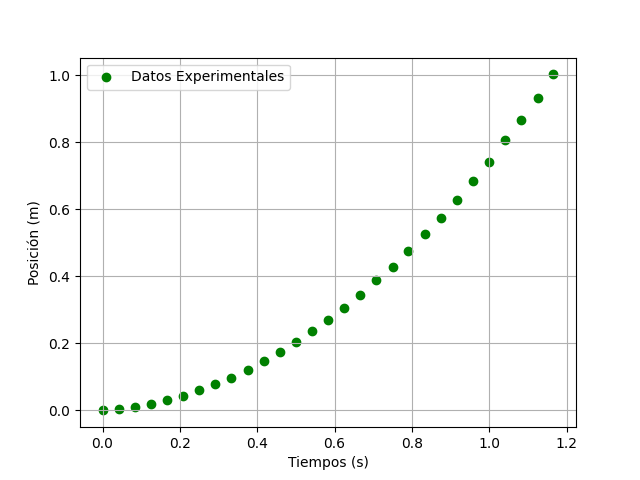
\includegraphics[scale=0.8]{50 g.png}
\caption{Grafica de la Tabla 3}
\end{figure}

\begin{figure}[h!]
\centering
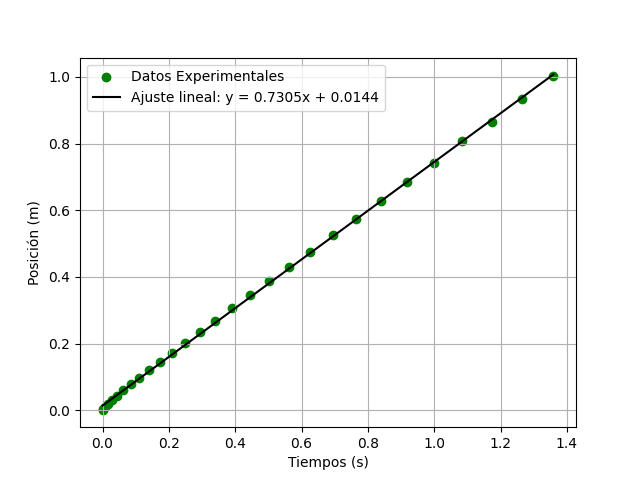
\includegraphics[scale=0.8]{50 g r.png}
\caption{Grafica de $t^2$ - posición con regresión lineal de la Tabla 3}
\end{figure}

\clearpage


Para la masa de 20 g\\

M = 0.2122 (0.0001) kg \\

m = 0.02 (0.0001) kg \\

mg = 0.196 (0.01) \\

a = 0.72 (0.05) \\

F = (0.72 $\frac{m}{s^2}$)(0.2122 kg) = 0.15 (0.01) N \\

Para la masa de 50 g\\

M = 0.2122 (0.0001) kg \\

m = 0.05 (0.0001) kg \\

mg = 0.491 (0.01) \\

a = 1.5 (0.07) \\

F = (1.5 $\frac{m}{s^2}$)(0.2122 kg) = 0.31 (0.01) N \\


\section{Discusión}

Como se puede notar en los resultados estos no son iguales a la aceleración de las masas, por lo que no sigue el modelo ideal, en este modelo real tendriamos que considerar una cuerda con masa que produce una fricción sobre la polea y un deslisador que sufre un rosamieto con el aire del riel. 

\section{Conclusión}

Aun en un riel de aire donde se desprecia la fricción, o en una cuerda donde se desprecia la masa, esta está presente y puede afectar el resultado final del experimento.  

\section{Referencias}

Miranda, Javier. (2025) \textit{Física Experimental. Introducción a los conceptos y métodos.} Recuperado el 18, 03, 2025, de https://copitarxives.fisica.unam.mx/LT0006ES/LT0006ES.pdf \\

Miranda, Javier. (2000). \textit{EVALUACIÓN DE LA INCERTIDUMBRE EN DATOS EXPERIMENTALES.} \\

Pérez, Héctor. (2018). \textit{Física general.}(Sexta Edición.). México: PATRIA educación \\

\end{document}